% Options for packages loaded elsewhere
\PassOptionsToPackage{unicode}{hyperref}
\PassOptionsToPackage{hyphens}{url}
\PassOptionsToPackage{dvipsnames,svgnames,x11names}{xcolor}
%
\documentclass[
  letterpaper,
  DIV=11,
  numbers=noendperiod]{scrartcl}

\usepackage{amsmath,amssymb}
\usepackage{iftex}
\ifPDFTeX
  \usepackage[T1]{fontenc}
  \usepackage[utf8]{inputenc}
  \usepackage{textcomp} % provide euro and other symbols
\else % if luatex or xetex
  \usepackage{unicode-math}
  \defaultfontfeatures{Scale=MatchLowercase}
  \defaultfontfeatures[\rmfamily]{Ligatures=TeX,Scale=1}
\fi
\usepackage{lmodern}
\ifPDFTeX\else  
    % xetex/luatex font selection
\fi
% Use upquote if available, for straight quotes in verbatim environments
\IfFileExists{upquote.sty}{\usepackage{upquote}}{}
\IfFileExists{microtype.sty}{% use microtype if available
  \usepackage[]{microtype}
  \UseMicrotypeSet[protrusion]{basicmath} % disable protrusion for tt fonts
}{}
\makeatletter
\@ifundefined{KOMAClassName}{% if non-KOMA class
  \IfFileExists{parskip.sty}{%
    \usepackage{parskip}
  }{% else
    \setlength{\parindent}{0pt}
    \setlength{\parskip}{6pt plus 2pt minus 1pt}}
}{% if KOMA class
  \KOMAoptions{parskip=half}}
\makeatother
\usepackage{xcolor}
\setlength{\emergencystretch}{3em} % prevent overfull lines
\setcounter{secnumdepth}{5}
% Make \paragraph and \subparagraph free-standing
\ifx\paragraph\undefined\else
  \let\oldparagraph\paragraph
  \renewcommand{\paragraph}[1]{\oldparagraph{#1}\mbox{}}
\fi
\ifx\subparagraph\undefined\else
  \let\oldsubparagraph\subparagraph
  \renewcommand{\subparagraph}[1]{\oldsubparagraph{#1}\mbox{}}
\fi

\usepackage{color}
\usepackage{fancyvrb}
\newcommand{\VerbBar}{|}
\newcommand{\VERB}{\Verb[commandchars=\\\{\}]}
\DefineVerbatimEnvironment{Highlighting}{Verbatim}{commandchars=\\\{\}}
% Add ',fontsize=\small' for more characters per line
\usepackage{framed}
\definecolor{shadecolor}{RGB}{241,243,245}
\newenvironment{Shaded}{\begin{snugshade}}{\end{snugshade}}
\newcommand{\AlertTok}[1]{\textcolor[rgb]{0.68,0.00,0.00}{#1}}
\newcommand{\AnnotationTok}[1]{\textcolor[rgb]{0.37,0.37,0.37}{#1}}
\newcommand{\AttributeTok}[1]{\textcolor[rgb]{0.40,0.45,0.13}{#1}}
\newcommand{\BaseNTok}[1]{\textcolor[rgb]{0.68,0.00,0.00}{#1}}
\newcommand{\BuiltInTok}[1]{\textcolor[rgb]{0.00,0.23,0.31}{#1}}
\newcommand{\CharTok}[1]{\textcolor[rgb]{0.13,0.47,0.30}{#1}}
\newcommand{\CommentTok}[1]{\textcolor[rgb]{0.37,0.37,0.37}{#1}}
\newcommand{\CommentVarTok}[1]{\textcolor[rgb]{0.37,0.37,0.37}{\textit{#1}}}
\newcommand{\ConstantTok}[1]{\textcolor[rgb]{0.56,0.35,0.01}{#1}}
\newcommand{\ControlFlowTok}[1]{\textcolor[rgb]{0.00,0.23,0.31}{#1}}
\newcommand{\DataTypeTok}[1]{\textcolor[rgb]{0.68,0.00,0.00}{#1}}
\newcommand{\DecValTok}[1]{\textcolor[rgb]{0.68,0.00,0.00}{#1}}
\newcommand{\DocumentationTok}[1]{\textcolor[rgb]{0.37,0.37,0.37}{\textit{#1}}}
\newcommand{\ErrorTok}[1]{\textcolor[rgb]{0.68,0.00,0.00}{#1}}
\newcommand{\ExtensionTok}[1]{\textcolor[rgb]{0.00,0.23,0.31}{#1}}
\newcommand{\FloatTok}[1]{\textcolor[rgb]{0.68,0.00,0.00}{#1}}
\newcommand{\FunctionTok}[1]{\textcolor[rgb]{0.28,0.35,0.67}{#1}}
\newcommand{\ImportTok}[1]{\textcolor[rgb]{0.00,0.46,0.62}{#1}}
\newcommand{\InformationTok}[1]{\textcolor[rgb]{0.37,0.37,0.37}{#1}}
\newcommand{\KeywordTok}[1]{\textcolor[rgb]{0.00,0.23,0.31}{#1}}
\newcommand{\NormalTok}[1]{\textcolor[rgb]{0.00,0.23,0.31}{#1}}
\newcommand{\OperatorTok}[1]{\textcolor[rgb]{0.37,0.37,0.37}{#1}}
\newcommand{\OtherTok}[1]{\textcolor[rgb]{0.00,0.23,0.31}{#1}}
\newcommand{\PreprocessorTok}[1]{\textcolor[rgb]{0.68,0.00,0.00}{#1}}
\newcommand{\RegionMarkerTok}[1]{\textcolor[rgb]{0.00,0.23,0.31}{#1}}
\newcommand{\SpecialCharTok}[1]{\textcolor[rgb]{0.37,0.37,0.37}{#1}}
\newcommand{\SpecialStringTok}[1]{\textcolor[rgb]{0.13,0.47,0.30}{#1}}
\newcommand{\StringTok}[1]{\textcolor[rgb]{0.13,0.47,0.30}{#1}}
\newcommand{\VariableTok}[1]{\textcolor[rgb]{0.07,0.07,0.07}{#1}}
\newcommand{\VerbatimStringTok}[1]{\textcolor[rgb]{0.13,0.47,0.30}{#1}}
\newcommand{\WarningTok}[1]{\textcolor[rgb]{0.37,0.37,0.37}{\textit{#1}}}

\providecommand{\tightlist}{%
  \setlength{\itemsep}{0pt}\setlength{\parskip}{0pt}}\usepackage{longtable,booktabs,array}
\usepackage{calc} % for calculating minipage widths
% Correct order of tables after \paragraph or \subparagraph
\usepackage{etoolbox}
\makeatletter
\patchcmd\longtable{\par}{\if@noskipsec\mbox{}\fi\par}{}{}
\makeatother
% Allow footnotes in longtable head/foot
\IfFileExists{footnotehyper.sty}{\usepackage{footnotehyper}}{\usepackage{footnote}}
\makesavenoteenv{longtable}
\usepackage{graphicx}
\makeatletter
\def\maxwidth{\ifdim\Gin@nat@width>\linewidth\linewidth\else\Gin@nat@width\fi}
\def\maxheight{\ifdim\Gin@nat@height>\textheight\textheight\else\Gin@nat@height\fi}
\makeatother
% Scale images if necessary, so that they will not overflow the page
% margins by default, and it is still possible to overwrite the defaults
% using explicit options in \includegraphics[width, height, ...]{}
\setkeys{Gin}{width=\maxwidth,height=\maxheight,keepaspectratio}
% Set default figure placement to htbp
\makeatletter
\def\fps@figure{htbp}
\makeatother

% load packages
\usepackage{geometry}
\usepackage{xcolor}
\usepackage{eso-pic}
\usepackage{fancyhdr}
\usepackage{sectsty}
\usepackage{fontspec}
\usepackage{titlesec}

%% Set page size with a wider right margin
\geometry{a4paper, total={170mm,257mm}, left=20mm, top=20mm, bottom=20mm, right=50mm}

%% Let's define some colours
\definecolor{light}{HTML}{E6E6FA}
\definecolor{highlight}{HTML}{800080}
\definecolor{dark}{HTML}{330033}

%% Let's add the border on the right hand side 
\AddToShipoutPicture{% 
    \AtPageLowerLeft{% 
        \put(\LenToUnit{\dimexpr\paperwidth-3cm},0){% 
            \color{light}\rule{3cm}{\LenToUnit\paperheight}%
          }%
     }%
     % logo
    \AtPageLowerLeft{% start the bar at the bottom right of the page
        \put(\LenToUnit{\dimexpr\paperwidth-2.25cm},27.2cm){% move it to the top right
            \color{light}
\includegraphics[width=1.5cm]{_extensions/nrennie/PrettyPDF/logo.png}
          }%
     }%
}

%% Style the page number
\fancypagestyle{mystyle}{
  \fancyhf{}
  \renewcommand\headrulewidth{0pt}
  \fancyfoot[R]{\thepage}
  \fancyfootoffset{3.5cm}
}
\setlength{\footskip}{20pt}

%% style the chapter/section fonts
\chapterfont{\color{dark}\fontsize{20}{16.8}\selectfont}
\sectionfont{\color{dark}\fontsize{20}{16.8}\selectfont}
\subsectionfont{\color{dark}\fontsize{14}{16.8}\selectfont}
\titleformat{\subsection}
  {\sffamily\Large\bfseries}{\thesection}{1em}{}[{\titlerule[0.8pt]}]
  
% left align title
\makeatletter
\renewcommand{\maketitle}{\bgroup\setlength{\parindent}{0pt}
\begin{flushleft}
  {\sffamily\huge\textbf{\MakeUppercase{\@title}}} \vspace{0.3cm} \newline
  {\Large {\@subtitle}} \newline
  \@author
\end{flushleft}\egroup
}
\makeatother

%% Use some custom fonts
\setsansfont{Ubuntu}[
    Path=_extensions/nrennie/PrettyPDF/Ubuntu/,
    Scale=0.9,
    Extension = .ttf,
    UprightFont=*-Regular,
    BoldFont=*-Bold,
    ItalicFont=*-Italic,
    ]

\setmainfont{Ubuntu}[
    Path=_extensions/nrennie/PrettyPDF/Ubuntu/,
    Scale=0.9,
    Extension = .ttf,
    UprightFont=*-Regular,
    BoldFont=*-Bold,
    ItalicFont=*-Italic,
    ]
\KOMAoption{captions}{tableheading}
\makeatletter
\@ifpackageloaded{tcolorbox}{}{\usepackage[skins,breakable]{tcolorbox}}
\@ifpackageloaded{fontawesome5}{}{\usepackage{fontawesome5}}
\definecolor{quarto-callout-color}{HTML}{909090}
\definecolor{quarto-callout-note-color}{HTML}{0758E5}
\definecolor{quarto-callout-important-color}{HTML}{CC1914}
\definecolor{quarto-callout-warning-color}{HTML}{EB9113}
\definecolor{quarto-callout-tip-color}{HTML}{00A047}
\definecolor{quarto-callout-caution-color}{HTML}{FC5300}
\definecolor{quarto-callout-color-frame}{HTML}{acacac}
\definecolor{quarto-callout-note-color-frame}{HTML}{4582ec}
\definecolor{quarto-callout-important-color-frame}{HTML}{d9534f}
\definecolor{quarto-callout-warning-color-frame}{HTML}{f0ad4e}
\definecolor{quarto-callout-tip-color-frame}{HTML}{02b875}
\definecolor{quarto-callout-caution-color-frame}{HTML}{fd7e14}
\makeatother
\makeatletter
\@ifpackageloaded{caption}{}{\usepackage{caption}}
\AtBeginDocument{%
\ifdefined\contentsname
  \renewcommand*\contentsname{Table of contents}
\else
  \newcommand\contentsname{Table of contents}
\fi
\ifdefined\listfigurename
  \renewcommand*\listfigurename{List of Figures}
\else
  \newcommand\listfigurename{List of Figures}
\fi
\ifdefined\listtablename
  \renewcommand*\listtablename{List of Tables}
\else
  \newcommand\listtablename{List of Tables}
\fi
\ifdefined\figurename
  \renewcommand*\figurename{Figure}
\else
  \newcommand\figurename{Figure}
\fi
\ifdefined\tablename
  \renewcommand*\tablename{Table}
\else
  \newcommand\tablename{Table}
\fi
}
\@ifpackageloaded{float}{}{\usepackage{float}}
\floatstyle{ruled}
\@ifundefined{c@chapter}{\newfloat{codelisting}{h}{lop}}{\newfloat{codelisting}{h}{lop}[chapter]}
\floatname{codelisting}{Listing}
\newcommand*\listoflistings{\listof{codelisting}{List of Listings}}
\makeatother
\makeatletter
\makeatother
\makeatletter
\@ifpackageloaded{caption}{}{\usepackage{caption}}
\@ifpackageloaded{subcaption}{}{\usepackage{subcaption}}
\makeatother
\makeatletter
\@ifpackageloaded{tcolorbox}{}{\usepackage[skins,breakable]{tcolorbox}}
\makeatother
\makeatletter
\@ifundefined{shadecolor}{\definecolor{shadecolor}{rgb}{.97, .97, .97}}{}
\makeatother
\makeatletter
\@ifundefined{codebgcolor}{\definecolor{codebgcolor}{named}{light}}{}
\makeatother
\makeatletter
\ifdefined\Shaded\renewenvironment{Shaded}{\begin{tcolorbox}[colback={codebgcolor}, enhanced, breakable, sharp corners, boxrule=0pt, frame hidden]}{\end{tcolorbox}}\fi
\makeatother
\ifLuaTeX
  \usepackage{selnolig}  % disable illegal ligatures
\fi
\usepackage{bookmark}

\IfFileExists{xurl.sty}{\usepackage{xurl}}{} % add URL line breaks if available
\urlstyle{same} % disable monospaced font for URLs
\hypersetup{
  pdftitle={Practical},
  colorlinks=true,
  linkcolor={highlight},
  filecolor={Maroon},
  citecolor={Blue},
  urlcolor={highlight},
  pdfcreator={LaTeX via pandoc}}

\title{Practical}
\author{}
\date{}

\begin{document}
\maketitle

\pagestyle{mystyle}

Start by loading usefull libraries:

\begin{Shaded}
\begin{Highlighting}[]
\FunctionTok{library}\NormalTok{(dplyr)}
\FunctionTok{library}\NormalTok{(INLA)}
\FunctionTok{library}\NormalTok{(ggplot2)}
\FunctionTok{library}\NormalTok{(patchwork)}
\FunctionTok{library}\NormalTok{(inlabru)     }
\CommentTok{\# load some libraries to generate nice map plots}
\FunctionTok{library}\NormalTok{(scico)}
\end{Highlighting}
\end{Shaded}

\textbf{Aim of this practical:} In this first practical we are going to
look at some simple models

\begin{enumerate}
\def\labelenumi{\arabic{enumi}.}
\tightlist
\item
  A \hyperref[Gaussian-link]{Gaussian model} with simulated data
\item
  A \hyperref[GLM-link]{GLM model with random effects}
\end{enumerate}

we are going to learn:

\begin{itemize}
\tightlist
\item
  How to fit a simple model with \texttt{inlabru}
\item
  How to explore the results
\item
  How to change the prior distributions
\item
  How to get predictions for missing data points
\end{itemize}

\subsection{Linear Model}\label{sec-linmodel}

As our first example we consider a simple linear regression model with
Gaussian observations \(y_i\sim\mathcal{N}(\mu_i, \sigma^2)\),
\(i = 1,\dots,N\) where \(\sigma^2\) is the observation error, and the
mean parameter \(\mu_i\) is linked to the linear predictor through an
identity function: \[
\eta_i = \mu_i = \beta_0 + \beta_1 x_i
\] where \(x_i\) is a covariate and \(\beta_0, \beta_1\) are parameters
to be estimated.

To finalize the Bayesian model we need to assign a \(\text{Gamma}(a,b)\)
prior to the precision parameter \(\tau = 1/\sigma^2\) and two
independent Gaussian priors with mean \(0\) and precision
\(\tau_{\beta}\) to the regression parameters \(\beta_0\) and
\(\beta_1\).

\begin{tcolorbox}[enhanced jigsaw, coltitle=black, left=2mm, breakable, rightrule=.15mm, opacitybacktitle=0.6, opacityback=0, colback=white, colbacktitle=quarto-callout-tip-color!10!white, bottomtitle=1mm, toptitle=1mm, title={Question}, titlerule=0mm, arc=.35mm, bottomrule=.15mm, colframe=quarto-callout-tip-color-frame, leftrule=.75mm, toprule=.15mm]

What is the dimension of the hyperparameter vector and latent Gaussian
field?

Answer

The hyperparameter vector has dimension 1, \(\pmb{\theta} = (\tau)\)
while the latent Gaussian field \(\pmb{u} = (\beta_0, \beta_1)\) has
dimension 2, \(0\) mean, and sparse precision matrix:

\[
\pmb{Q} = \tau_{\beta}\begin{bmatrix}
1 & 0\\
0 & 1
\end{bmatrix}
\]

\end{tcolorbox}

\begin{tcolorbox}[enhanced jigsaw, coltitle=black, left=2mm, breakable, rightrule=.15mm, opacitybacktitle=0.6, opacityback=0, colback=white, colbacktitle=quarto-callout-note-color!10!white, bottomtitle=1mm, toptitle=1mm, title=\textcolor{quarto-callout-note-color}{\faInfo}\hspace{0.5em}{Note}, titlerule=0mm, arc=.35mm, bottomrule=.15mm, colframe=quarto-callout-note-color-frame, leftrule=.75mm, toprule=.15mm]

We can write the linear predictor vector
\(\pmb{\eta} = (\eta_i,\dots,\eta_N)\) as

\[
\pmb{\eta} = \pmb{A}\pmb{u} = \pmb{A}_1\pmb{u}_1 + \pmb{A}_2\pmb{u}_2 = \begin{bmatrix}
1 \\
1\\
\vdots\\
1
\end{bmatrix} \beta_0 + \begin{bmatrix}
x_1 \\
x_2\\
\vdots\\
x_N
\end{bmatrix} \beta_1
\]

Our linear predictor consists then of two components.

\end{tcolorbox}

\subsubsection{\texorpdfstring{\textbf{Simulate example
data}}{Simulate example data}}\label{simulate-example-data}

\begin{center}\rule{0.5\linewidth}{0.5pt}\end{center}

In this practical we will use simulated Gaussian data to get familiar
with the \texttt{inlabru} workflow. Moreover, we will see how to change
the prior distributions both for the fixed effects \(\beta_0\) and
\(\beta_1\) and for the hyperparameter \(\tau = 1/\sigma^2\). First, we
simulate data from the model

\[
y_i\sim\mathcal{N}(\eta_i,0.1^2), \ i = 1,\dots,100
\]

with

\[
\eta_i = \beta_0 + \beta_1 x_i
\]

where \(\beta_0 = 2\),\(\beta_1 = 0.5\) and the values of the covariate
\(x\) are generated from an Uniform(0,1) distribution. The simulated
response and covariate data are then saved in a \texttt{data.frame}
object.

\begin{Shaded}
\begin{Highlighting}[]
\NormalTok{beta }\OtherTok{=} \FunctionTok{c}\NormalTok{(}\DecValTok{1}\NormalTok{,}\DecValTok{1}\NormalTok{)}
\NormalTok{sd\_error }\OtherTok{=} \DecValTok{1}

\NormalTok{n }\OtherTok{=} \DecValTok{100}
\NormalTok{x }\OtherTok{=} \FunctionTok{rnorm}\NormalTok{(n)}
\NormalTok{y }\OtherTok{=}\NormalTok{ beta[}\DecValTok{1}\NormalTok{] }\SpecialCharTok{+}\NormalTok{ beta[}\DecValTok{2}\NormalTok{] }\SpecialCharTok{*}\NormalTok{ x }\SpecialCharTok{+} \FunctionTok{rnorm}\NormalTok{(n, }\AttributeTok{sd =}\NormalTok{ sd\_error)}

\NormalTok{df }\OtherTok{=} \FunctionTok{data.frame}\NormalTok{(}\AttributeTok{y =}\NormalTok{ y, }\AttributeTok{x =}\NormalTok{ x)  }
\end{Highlighting}
\end{Shaded}

\subsubsection{\texorpdfstring{\textbf{Fitting a linear regression model
with
\texttt{inlabru}}}{Fitting a linear regression model with inlabru}}\label{fitting-a-linear-regression-model-with-inlabru}

\begin{center}\rule{0.5\linewidth}{0.5pt}\end{center}

\textbf{Defining model components}

The model has two parameters to be estimated \(\beta_1\) and
\(\beta_2\). We need to define the two corresponding model components:

\begin{Shaded}
\begin{Highlighting}[]
\NormalTok{cmp }\OtherTok{=}  \ErrorTok{\textasciitilde{}} \FunctionTok{Intercept}\NormalTok{(}\DecValTok{1}\NormalTok{) }\SpecialCharTok{+} \FunctionTok{beta\_1}\NormalTok{(x, }\AttributeTok{model =} \StringTok{"linear"}\NormalTok{)}
\end{Highlighting}
\end{Shaded}

The \texttt{cmp} object is here used to define model components. We can
give them any useful names we like

\begin{tcolorbox}[enhanced jigsaw, coltitle=black, left=2mm, breakable, rightrule=.15mm, opacitybacktitle=0.6, opacityback=0, colback=white, colbacktitle=quarto-callout-note-color!10!white, bottomtitle=1mm, toptitle=1mm, title=\textcolor{quarto-callout-note-color}{\faInfo}\hspace{0.5em}{Note}, titlerule=0mm, arc=.35mm, bottomrule=.15mm, colframe=quarto-callout-note-color-frame, leftrule=.75mm, toprule=.15mm]

Note that \texttt{Intercept()} is one of \texttt{inlabru} special names
and it is used to define a global intercept. You should explicitly
exclude automatic intercept when not using the special
\texttt{Intercept} name, e.g.

\begin{Shaded}
\begin{Highlighting}[]
\NormalTok{cmp }\OtherTok{=}  \ErrorTok{\textasciitilde{}} \SpecialCharTok{{-}}\DecValTok{1} \SpecialCharTok{+} \FunctionTok{myIntercept}\NormalTok{(}\DecValTok{1}\NormalTok{) }\SpecialCharTok{+} \FunctionTok{beta\_1}\NormalTok{(x, }\AttributeTok{model =} \StringTok{"linear"}\NormalTok{)}
\end{Highlighting}
\end{Shaded}

\end{tcolorbox}

\textbf{Observation model construction}

The next step is to construct the observation model by defining the
model likelihood. The most important inputs here are the
\texttt{formula}, the \texttt{family} and the \texttt{data}.

The \texttt{formula} defines how the components should be combined in
order to define the model predictor.

\begin{Shaded}
\begin{Highlighting}[]
\NormalTok{formula }\OtherTok{=}\NormalTok{ y }\SpecialCharTok{\textasciitilde{}}\NormalTok{ Intercept }\SpecialCharTok{+}\NormalTok{ beta\_1}
\end{Highlighting}
\end{Shaded}

\begin{tcolorbox}[enhanced jigsaw, coltitle=black, left=2mm, breakable, rightrule=.15mm, opacitybacktitle=0.6, opacityback=0, colback=white, colbacktitle=quarto-callout-note-color!10!white, bottomtitle=1mm, toptitle=1mm, title=\textcolor{quarto-callout-note-color}{\faInfo}\hspace{0.5em}{Note}, titlerule=0mm, arc=.35mm, bottomrule=.15mm, colframe=quarto-callout-note-color-frame, leftrule=.75mm, toprule=.15mm]

In this case we can also use the shortcut
\texttt{formula\ =\ y\ \textasciitilde{}\ .}. This will tell
\texttt{inlarbu} that the model is linear and that it is not necessary
to linearize the model and assess convergence.

\end{tcolorbox}

The likelihood is defined using the \texttt{bru\_obs()} function as
follows:

\begin{Shaded}
\begin{Highlighting}[]
\NormalTok{lik }\OtherTok{=}  \FunctionTok{bru\_obs}\NormalTok{(}\AttributeTok{formula =}\NormalTok{ y }\SpecialCharTok{\textasciitilde{}}\NormalTok{.,}
            \AttributeTok{family =} \StringTok{"gaussian"}\NormalTok{,}
            \AttributeTok{data =}\NormalTok{ df)}
\end{Highlighting}
\end{Shaded}

\textbf{Fit the model}

We fit the model using the \texttt{bru()} functions which takes as input
the components and the observation model:

\begin{Shaded}
\begin{Highlighting}[]
\NormalTok{fit.lm }\OtherTok{=} \FunctionTok{bru}\NormalTok{(cmp, lik)}
\end{Highlighting}
\end{Shaded}

The \texttt{summary()} function will give access to some basic
information about model fit and estimates

\begin{Shaded}
\begin{Highlighting}[]
\FunctionTok{summary}\NormalTok{(fit.lm)}
\end{Highlighting}
\end{Shaded}

\begin{verbatim}
inlabru version: 2.12.0
INLA version: 25.02.10
Components:
Intercept: main = linear(1), group = exchangeable(1L), replicate = iid(1L), NULL
beta_1: main = linear(x), group = exchangeable(1L), replicate = iid(1L), NULL
Likelihoods:
  Family: 'gaussian'
    Tag: ''
    Data class: 'data.frame'
    Response class: 'numeric'
    Predictor: y ~ .
    Used components: effects[Intercept, beta_1], latent[]
Time used:
    Pre = 0.383, Running = 0.182, Post = 0.0761, Total = 0.642 
Fixed effects:
           mean    sd 0.025quant 0.5quant 0.975quant  mode kld
Intercept 0.981 0.099      0.787    0.981      1.175 0.981   0
beta_1    1.120 0.103      0.917    1.120      1.322 1.120   0

Model hyperparameters:
                                        mean    sd 0.025quant 0.5quant
Precision for the Gaussian observations 1.04 0.148      0.776     1.04
                                        0.975quant mode
Precision for the Gaussian observations       1.35 1.02

Deviance Information Criterion (DIC) ...............: 285.35
Deviance Information Criterion (DIC, saturated) ....: 105.43
Effective number of parameters .....................: 3.00

Watanabe-Akaike information criterion (WAIC) ...: 285.24
Effective number of parameters .................: 2.79

Marginal log-Likelihood:  -162.09 
 is computed 
Posterior summaries for the linear predictor and the fitted values are computed
(Posterior marginals needs also 'control.compute=list(return.marginals.predictor=TRUE)')
\end{verbatim}

We can see that both the intercept and slope and the error precision are
correctly estimated. We can then plot the marginal posterior for
\(\beta_0\) as follows:

\begin{Shaded}
\begin{Highlighting}[]
\FunctionTok{plot}\NormalTok{(fit.lm, }\StringTok{"Intercept"}\NormalTok{)}
\end{Highlighting}
\end{Shaded}

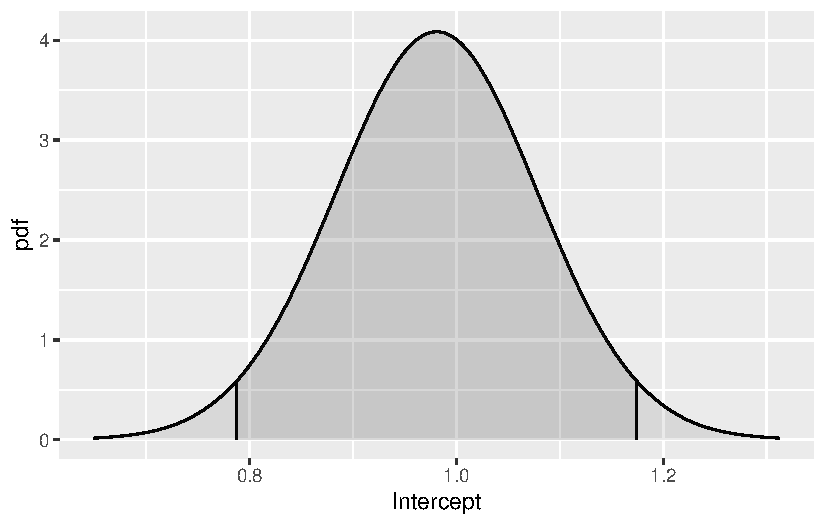
\includegraphics{test_files/figure-pdf/unnamed-chunk-10-1.pdf}

\begin{tcolorbox}[enhanced jigsaw, coltitle=black, left=2mm, breakable, rightrule=.15mm, opacitybacktitle=0.6, opacityback=0, colback=white, colbacktitle=quarto-callout-warning-color!10!white, bottomtitle=1mm, toptitle=1mm, title={Task}, titlerule=0mm, arc=.35mm, bottomrule=.15mm, colframe=quarto-callout-warning-color-frame, leftrule=.75mm, toprule=.15mm]

Plot the posterior marginals for \(\beta_1\) and for the precision of
the observation error \(\pi(\tau|y)\)

Take hint

See the \texttt{summary()} output to check the names for the different
model components.

Click here to see the solution

\begin{Shaded}
\begin{Highlighting}[]
\FunctionTok{plot}\NormalTok{(fit.lm, }\StringTok{"beta\_1"}\NormalTok{) }\SpecialCharTok{+}
\FunctionTok{plot}\NormalTok{(fit.lm, }\StringTok{"Precision for the Gaussian observations"}\NormalTok{)}
\end{Highlighting}
\end{Shaded}

\begin{center}
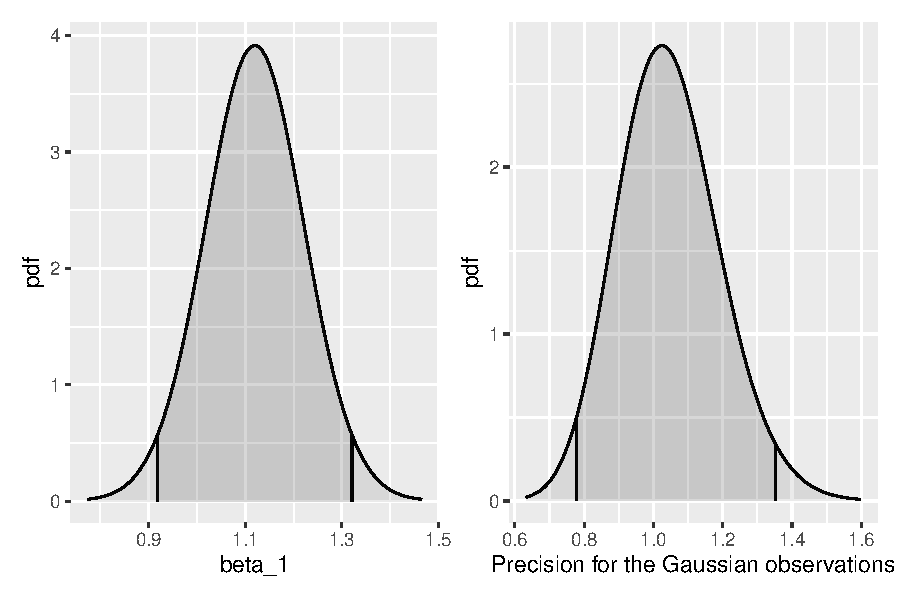
\includegraphics{test_files/figure-pdf/unnamed-chunk-11-1.pdf}
\end{center}

\end{tcolorbox}

\begin{tcolorbox}[enhanced jigsaw, coltitle=black, left=2mm, breakable, rightrule=.15mm, opacitybacktitle=0.6, opacityback=0, colback=white, colbacktitle=quarto-callout-warning-color!10!white, bottomtitle=1mm, toptitle=1mm, title={Task}, titlerule=0mm, arc=.35mm, bottomrule=.15mm, colframe=quarto-callout-warning-color-frame, leftrule=.75mm, toprule=.15mm]

Plot the fitted values with 95\% Credible intervals.

Take hint

\texttt{bru} objects information about the linear predictor can be
accessed through \texttt{fit.lm\$summary.fitted.values}.

Click here to see the solution

\begin{Shaded}
\begin{Highlighting}[]
\NormalTok{df }\SpecialCharTok{\%\textgreater{}\%} \FunctionTok{mutate}\NormalTok{(}\AttributeTok{post\_mean =}\NormalTok{ fit.lm}\SpecialCharTok{$}\NormalTok{summary.fitted.values[}\DecValTok{1}\SpecialCharTok{:}\DecValTok{100}\NormalTok{,}\StringTok{"mean"}\NormalTok{],}
              \AttributeTok{q25 =}\NormalTok{ fit.lm}\SpecialCharTok{$}\NormalTok{summary.fitted.values[}\DecValTok{1}\SpecialCharTok{:}\DecValTok{100}\NormalTok{,}\StringTok{"0.025quant"}\NormalTok{],}
              \AttributeTok{q975 =}\NormalTok{ fit.lm}\SpecialCharTok{$}\NormalTok{summary.fitted.values[}\DecValTok{1}\SpecialCharTok{:}\DecValTok{100}\NormalTok{,}\StringTok{"0.975quant"}\NormalTok{])}\SpecialCharTok{\%\textgreater{}\%}
  \FunctionTok{ggplot}\NormalTok{()}\SpecialCharTok{+}\FunctionTok{geom\_point}\NormalTok{(}\FunctionTok{aes}\NormalTok{(}\AttributeTok{x=}\NormalTok{x,}\AttributeTok{y=}\NormalTok{y),}\AttributeTok{alpha=}\FloatTok{0.5}\NormalTok{,}\AttributeTok{color=}\StringTok{"grey40"}\NormalTok{)}\SpecialCharTok{+}
  \FunctionTok{geom\_line}\NormalTok{(}\FunctionTok{aes}\NormalTok{(}\AttributeTok{x=}\NormalTok{x,}\AttributeTok{y=}\NormalTok{post\_mean),}\AttributeTok{col=}\DecValTok{2}\NormalTok{)}\SpecialCharTok{+}
  \FunctionTok{geom\_ribbon}\NormalTok{(}\FunctionTok{aes}\NormalTok{(}\AttributeTok{x =}\NormalTok{ x, }\AttributeTok{ymax =}\NormalTok{ q975, }\AttributeTok{ymin =}\NormalTok{ q25),}\AttributeTok{fill=}\StringTok{"tomato"}\NormalTok{, }\AttributeTok{alpha =} \FloatTok{0.3}\NormalTok{)}
\end{Highlighting}
\end{Shaded}

\begin{center}
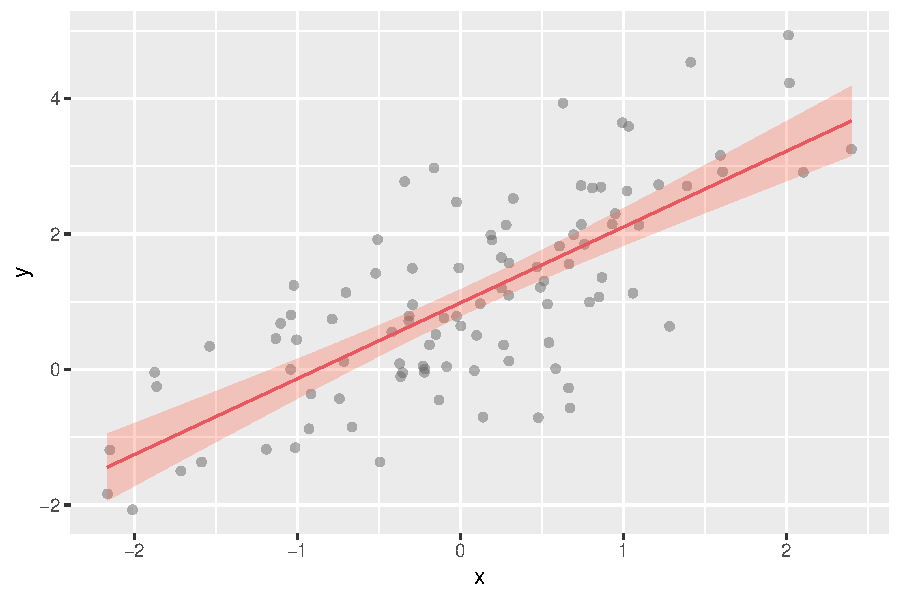
\includegraphics{test_files/figure-pdf/unnamed-chunk-12-1.pdf}
\end{center}

\end{tcolorbox}

\subsubsection{Generate model
predictions}\label{generate-model-predictions}

\begin{center}\rule{0.5\linewidth}{0.5pt}\end{center}

Now we can take the fitted \texttt{bru} object and use the
\texttt{predict} function to produce predictions given a new set of
values for the model covariates or the original values used for the
model fit

\begin{Shaded}
\begin{Highlighting}[]
\NormalTok{new\_data }\OtherTok{=} \FunctionTok{data.frame}\NormalTok{(}\AttributeTok{x =} \FunctionTok{c}\NormalTok{(df}\SpecialCharTok{$}\NormalTok{x, }\FunctionTok{runif}\NormalTok{(}\DecValTok{10}\NormalTok{)),}
                      \AttributeTok{y =} \FunctionTok{c}\NormalTok{(df}\SpecialCharTok{$}\NormalTok{y, }\FunctionTok{rep}\NormalTok{(}\ConstantTok{NA}\NormalTok{,}\DecValTok{10}\NormalTok{)))}
\NormalTok{pred }\OtherTok{=} \FunctionTok{predict}\NormalTok{(fit.lm, new\_data, }\SpecialCharTok{\textasciitilde{}}\NormalTok{ Intercept }\SpecialCharTok{+}\NormalTok{ beta\_1)}
\end{Highlighting}
\end{Shaded}

\subsection{Plot}

\begin{figure}[H]

{\centering 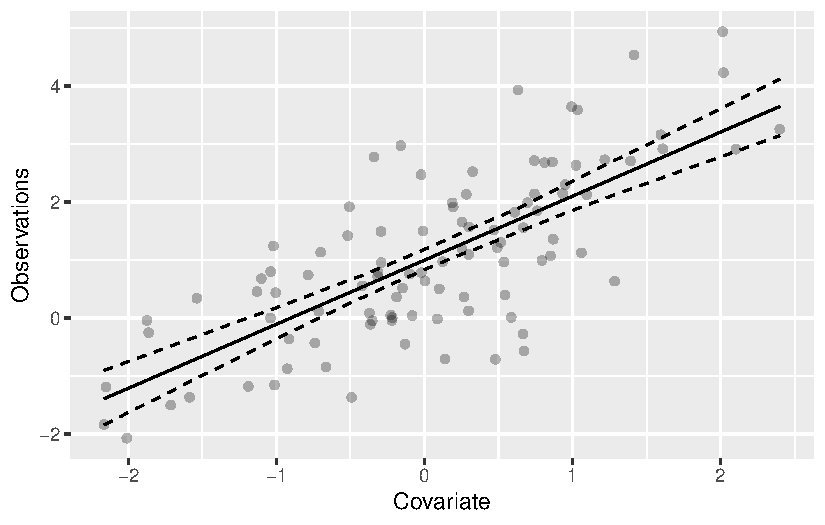
\includegraphics{test_files/figure-pdf/unnamed-chunk-14-1.pdf}

}

\caption{Data and 95\% credible intervals}

\end{figure}%

\subsection{R Code}

\begin{Shaded}
\begin{Highlighting}[]
\NormalTok{pred }\SpecialCharTok{\%\textgreater{}\%} \FunctionTok{ggplot}\NormalTok{() }\SpecialCharTok{+} 
  \FunctionTok{geom\_point}\NormalTok{(}\FunctionTok{aes}\NormalTok{(x,y), }\AttributeTok{alpha =} \FloatTok{0.3}\NormalTok{) }\SpecialCharTok{+}
  \FunctionTok{geom\_line}\NormalTok{(}\FunctionTok{aes}\NormalTok{(x,mean)) }\SpecialCharTok{+}
  \FunctionTok{geom\_line}\NormalTok{(}\FunctionTok{aes}\NormalTok{(x, q0}\FloatTok{.025}\NormalTok{), }\AttributeTok{linetype =} \StringTok{"dashed"}\NormalTok{)}\SpecialCharTok{+}
  \FunctionTok{geom\_line}\NormalTok{(}\FunctionTok{aes}\NormalTok{(x, q0}\FloatTok{.975}\NormalTok{), }\AttributeTok{linetype =} \StringTok{"dashed"}\NormalTok{)}\SpecialCharTok{+}
  \FunctionTok{xlab}\NormalTok{(}\StringTok{"Covariate"}\NormalTok{) }\SpecialCharTok{+} \FunctionTok{ylab}\NormalTok{(}\StringTok{"Observations"}\NormalTok{)}
\end{Highlighting}
\end{Shaded}




\end{document}
